\documentclass[journal,12pt,onecolumn]{IEEEtran}
\usepackage{cite}
\usepackage{graphicx}
\usepackage{amsmath,amssymb,amsfonts,amsthm}
\usepackage{algorithmic}
\usepackage{graphicx}
\usepackage{textcomp}
\usepackage{xcolor}
\usepackage{txfonts}
\usepackage{listings}
\usepackage{enumitem}
\usepackage{mathtools}
\usepackage{gensymb}
\usepackage{comment}
\usepackage[breaklinks=true]{hyperref}
\usepackage{tkz-euclide} 
\usepackage{listings}
\usepackage{gvv}                                        
\usepackage[latin1]{inputenc} 
\usetikzlibrary{arrows.meta, positioning}
\usepackage{xparse}
\usepackage{color}                                            
\usepackage{array}                                            
\usepackage{longtable}                                       
\usepackage{calc}                                             
\usepackage{multirow}
\usepackage{multicol}
\usepackage{hhline}                                           
\usepackage{ifthen}                                           
\usepackage{lscape}
\usepackage{tabularx}
\usepackage{array}
\usepackage{float}
\newtheorem{theorem}{Theorem}[section]
\newtheorem{problem}{Problem}
\newtheorem{proposition}{Proposition}[section]
\newtheorem{lemma}{Lemma}[section]
\newtheorem{corollary}[theorem]{Corollary}
\newtheorem{example}{Example}[section]
\newtheorem{definition}[problem]{Definition}
\newcommand{\BEQA}{\begin{eqnarray}}
\newcommand{\EEQA}{\end{eqnarray}}
\usepackage{float}
\theoremstyle{remark}
\usepackage{circuitikz}
\usepackage{tikz}
\title{GG1: GEOLOGY AND GEOPHYSICS}
\author{EE25BTECH11032- KARTIK LAHOTI}
\begin{document}

\maketitle

\begin{enumerate}

\item Is there any good show \rule{3cm}{0.15mm} television tonight?
Select the most appropriate option to complete the above sentence. \hfill{\brak{\text{GATE GG-1 2025}}}
\begin{enumerate}
    \begin{multicols}{4}
    \item in
    \item at
    \item within
    \item on
    \end{multicols}
\end{enumerate}

\item As the police officer was found guilty of embezzlement, he was \rule{3cm}{0.15mm} dismissed from the service in accordance with the Service Rules.
Select the most appropriate option to complete the above sentence. \hfill{\brak{\text{GATE GG-1 2025}}}
\begin{enumerate}
    \begin{multicols}{4}
    \item sumptuously
    \item brazenly
    \item unintentionally
    \item summarily
    \end{multicols}
\end{enumerate}

\item The sum of the following infinite series is:
\begin{align*}
\frac{1}{1!} + \frac{1}{2!} + \frac{1}{3!} + \frac{1}{4!} + \frac{1}{5!} + \cdots
\end{align*}
\hfill{\brak{\text{GATE GG-1 2025}}}
\begin{enumerate}
    \begin{multicols}{4}
    \item $\pi$
    \item $1+e$
    \item $e-1$
    \item $e$
    \end{multicols}
\end{enumerate}

\item A thin wire is used to construct all the edges of a cube of $1\,m$ side by bending, cutting and soldering the wire. If the wire is $12\,m$ long, what is the minimum number of cuts required to construct the wire frame to form the cube? \hfill{\brak{\text{GATE GG-1 2025}}}
\begin{enumerate}
    \begin{multicols}{4}
    \item $3$
    \item $4$
    \item $6$
    \item $12$
    \end{multicols}
\end{enumerate}

\item The figures I, II and III are parts of a sequence. Which one of the following options comes next in the sequence at IV?
\begin{figure}[H]
    \centering
    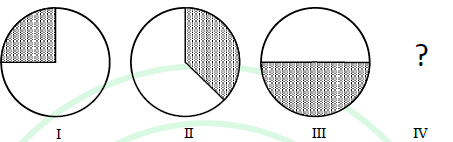
\includegraphics[width=0.8\columnwidth]{figs/fig1.png}
    \caption{}
    \label{fig:q5}
\end{figure}
\hfill{\brak{\text{GATE GG-1 2025}}}
\begin{enumerate}
\begin{multicols}{2}
    \item 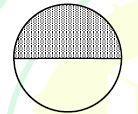
\includegraphics[width=0.2\columnwidth]{figs/fig1a.png} 
    \item 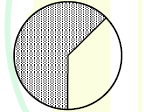
\includegraphics[width=0.2\columnwidth]{figs/fig1b.png} 
    \item 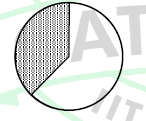
\includegraphics[width=0.2\columnwidth]{figs/fig1c.png} 
    \item 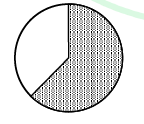
\includegraphics[width=0.2\columnwidth]{figs/fig1d.png}
\end{multicols}
\end{enumerate}

\item "Why do they pull down and do away with crooked streets, I wonder, which are my delight, and hurt no man living? Every day the wealthier nations are pulling down one or another in their capitals and their great towns: they do not know why they do it; neither do I. It ought to be enough, surely, to drive the great broad ways which commerce needs and which are the life-channels of a modern city, without destroying all history and all the humanity in between: the islands of the past." \brak{\text{From Hilaire Belloc's "The Crooked Streets"}}
Based only on the information provided in the above passage, which one of the following statements is true? \hfill{\brak{\text{GATE GG-1 2025}}}
\begin{enumerate}
    \item The author of the passage takes delight in wondering.
    \item The wealthier nations are pulling down the crooked streets in their capitals.
    \item In the past, crooked streets were only built on islands.
    \item Great broad ways are needed to protect commerce and history.
\end{enumerate}

\item Rohit goes to a restaurant for lunch at about $1$ PM. When he enters the restaurant, he notices that the hour and minute hands on the wall clock are exactly coinciding. After about an hour, when he leaves the restaurant, he notices that the clock hands are again exactly coinciding. How much time \brak{\text{in minutes}} did Rohit spend at the restaurant? \hfill{\brak{\text{GATE GG-1 2025}}}
\begin{enumerate}
\begin{multicols}{2}
    \item $64\frac{6}{11}$
    \item $66\frac{5}{13}$
    \item $65\frac{5}{11}$
    \item $66\frac{6}{13}$
    
\end{multicols}    
\end{enumerate}

\item A color model is shown in the figure with color codes: Yellow \brak{Y}, Magenta \brak{M}, Cyan \brak{Cy}, Red \brak{R}, Blue \brak{Bl}, Green \brak{G}, and Black \brak{K}.
\begin{figure}[H]
    \centering
    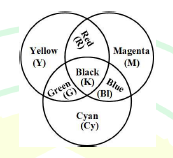
\includegraphics[width=0.5\columnwidth]{figs/fig2.png}
    \caption{}
    \label{fig:q8}
\end{figure}
Which one of the following options displays the color codes that are consistent with the color model? \hfill{\brak{\text{GATE GG-1 2025}}}
\begin{enumerate}
\begin{multicols}{2}
    \item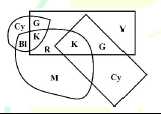
\includegraphics[width=0.4\columnwidth]{figs/fig2a.png}
    \item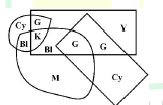
\includegraphics[width=0.4\columnwidth]{figs/fig2b.png}
    \item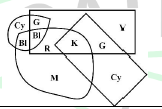
\includegraphics[width=0.4\columnwidth]{figs/fig2c.png}
    \item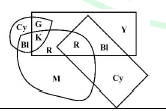
\includegraphics[width=0.4\columnwidth]{figs/fig2d.png}
\end{multicols} 
\end{enumerate}

\item A circle with center at $\brak{x,y}=\brak{0.5,0}$ and radius $=0.5$ intersects with another circle with center at $\brak{x,y}=\brak{1,1}$ and radius $=1$ at two points. One of the points of intersection $\brak{x, y}$ is: \hfill{\brak{\text{GATE GG-1 2025}}}
\begin{enumerate}
    \begin{multicols}{4}
    \item $\brak{0,0}$
    \item $\brak{0.2, 0.4}$
    \item $\brak{0.5, 0.5}$
    \item $\brak{1,2}$
    \end{multicols}
\end{enumerate}

\item An object is said to have an n-fold rotational symmetry if the object, rotated by an angle of $\frac{2\pi}{n}$, is identical to the original. Which one of the following objects exhibits $4$-fold rotational symmetry about an axis perpendicular to the plane of the screen? Note: The figures shown are representative. \hfill{\brak{\text{GATE GG-1 2025}}}
\begin{enumerate}
\begin{multicols}{2}
    \item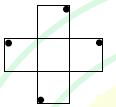
\includegraphics[width=0.4\columnwidth]{figs/fig3a.png}
    \item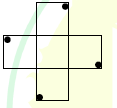
\includegraphics[width=0.4\columnwidth]{figs/fig3b.png}
    \item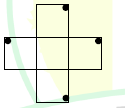
\includegraphics[width=0.4\columnwidth]{figs/fig3c.png}
    \item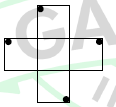
\includegraphics[width=0.4\columnwidth]{figs/fig3d.png}
\end{multicols}
\end{enumerate}

\item The most volcanically active body in our Solar System is  \hfill{\brak{\text{GATE GG-1 2025}}}
\begin{enumerate}
    \begin{multicols}{4}
    \item Mars
    \item Io
    \item Moon
    \item Venus
    \end{multicols}
\end{enumerate}

\item A type of fold which is relatively sharp and angular at its synformal and antiformal hinges is known as  \hfill{\brak{\text{GATE GG-1 2025}}}
\begin{enumerate}
    \begin{multicols}{4}
    \item Drag fold
    \item Chevron fold
    \item Dome
    \item Basin
    \end{multicols}
\end{enumerate}

\item Which one of the following geophysical methods can provide information on deep Earth structures $\brak{\text{of the order of }1000\,km}$ with highest resolution? \hfill{\brak{\text{GATE GG-1 2025}}}
\begin{enumerate}
    \begin{multicols}{2}
    \item Seismic methods
    \item Magnetic methods
    \item Electrical methods
    \item Gravity methods
    \end{multicols}
\end{enumerate}

\item The continuous series of Bowen's reaction series is represented by  \hfill{\brak{\text{GATE GG-1 2025}}}
\begin{enumerate}
    \item the orthoclase - albite feldspar system
    \item the anorthite - albite system
    \item the forsterite - fayalite system
    \item the diopside - anorthite system
\end{enumerate}

\item Which of the following time boundaries correspond\brak{s} to major mass extinction events? \hfill{\brak{\text{GATE GG-1 2025}}}
\begin{enumerate}
    \item Cretaceous - Paleogene
    \item Paleogene - Neogene
    \item Permian Triassic
    \item Precambrian - Cambrian
\end{enumerate}

\item A watershed has an area of $74 \text{ km}^2$. The stream network within this watershed consists of three different stream orders. The stream lengths in each order are as follows: 

$I^{st}$ order streams: $3\,km$ km, $2.5\,km$, $4\,km$, $3\,km$, $2\,km$, $5\,km$ 

$II^{nd}$ order streams: $10\,km$, $15\,km$, $7\,km$ 

$III^{rd}$ order streams: $30\,km$ 

The drainage density of the watershed is \rule{3cm}{0.15mm} $\text{km/km}^2$. \brak{\text{Round off to two decimal places}} \hfill{\brak{\text{GATE GG-1 2025}}}

\item A sample contains $7\, wt\,\%\,CaO$ and $5\, wt\,\%\,MgO$. The molar ratio of $CaO$ to $MgO$ in the sample is \rule{3cm}{0.15mm}. \brak{\text{Round off to two decimal places}} \hfill{\brak{\text{GATE GG-1 2025}}}

\item Select the option that lists oxide minerals only. \hfill{\brak{\text{GATE GG-1 2025}}}
\begin{enumerate}
    \item Spinel, Corundum, Rutile
    \item Olivine, Pyroxene, Magnetite
    \item Apatite, Galena, Monazite
    \item Fluorite, Halite, Calcite
\end{enumerate}

\item Consider two intersecting, north-easterly striking and south-easterly dipping dikes Y1 and Y2, which are exposed on an east-west trending vertical wall of a granite \brak{X} quarry as shown below.
\begin{figure}[H]
    \centering
    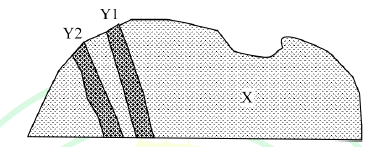
\includegraphics[width=0.5\columnwidth]{figs/fig4.png}
    \caption{}
    \label{fig:q19}
\end{figure}
The angle that the dikes make with the horizontal on the quarry wall is \rule{3cm}{0.15mm} \hfill{\brak{\text{GATE GG-1 2025}}}
\begin{enumerate}
\begin{multicols}{2}
    \item true dip
    \item apparent dip
    \item rake
    \item attitude of foliation
\end{multicols}
\end{enumerate}

\item The ratio of P-wave to S-wave velocities, $V_p/V_s$, within the Earth depends on \rule{3cm}{0.15mm} \hfill{\brak{\text{GATE GG-1 2025}}}
\begin{enumerate}
\begin{multicols}{2}
    \item bulk modulus
    \item shear modulus
    \item density
    \item coefficient of internal friction
\end{multicols}
\end{enumerate}

\item Three pixels P, Q, and R in an image are characterized by the NDVI values of $+0.84$, $+0.01$, and $-0.89$, respectively. Which of the following options is/are correct? \hfill{\brak{\text{GATE GG-1 2025}}}
\begin{enumerate}
    \item P is from vegetation area and Q is from barren land
    \item Q is from water body and R is from barren land
    \item Q is from barren land and R is from water body
    \item P is from vegetation area and Q is from water body
\end{enumerate}

\item Which of the following can indicate the presence of significant sub-surface iron mineralization? \hfill{\brak{\text{GATE GG-1 2025}}}
\begin{enumerate}
    \item Free air gravity anomaly
    \item Bouguer gravity anomaly
    \item Magnetic anomaly
    \item Electrical resistivity measurements
\end{enumerate}

\item Which of the following statements is/are correct regarding the magnetic field lines of the Earth, at the magnetic poles and the magnetic equator? \hfill{\brak{\text{GATE GG-1 2025}}}
\begin{enumerate}
    \item Horizonal at the equator
    \item Vertical at the poles
    \item Horizonal at the poles
    \item Vertical at the equator
\end{enumerate}

\item If the lowest Digital Number \brak{DN} value in an image of $10$-bit radiometric resolution is $0$, then the maximum DN value of that image is \rule{3cm}{0.15mm}. \brak{\text{Answer in integer}} \hfill{\brak{\text{GATE GG-1 2025}}}

\item If one liter of water at pH $7$ is mixed with one liter of water at pH $6$, the resulting pH of the mixture is \rule{3cm}{0.15mm}. \brak{\text{Round off to two decimal places}} \hfill{\brak{\text{GATE GG-1 2025}}}

\item A hillslope is shown below. If the area over the failure plane is $50 \text{ m}^2$ and the weight of the hillslope material \brak{W} is $2000$ tons, the Factor of Safety \brak{FOS} for this hillslope in dry conditions is \rule{3cm}{0.15mm}. \brak{\text{Cohesion along failure plane $=196$ KPa, dip of failure plane $=60\degree$, and internal friction angle $=30\degree$}}. \brak{\text{Round off to two decimal places}}
\begin{figure}[H]
    \centering
    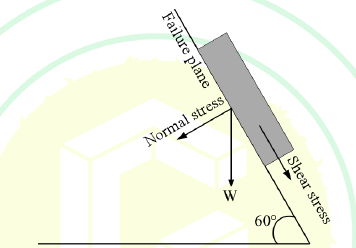
\includegraphics[width=0.5\columnwidth]{figs/fig5.png}
    \caption{}
    \label{fig:q26}
\end{figure}
\hfill{\brak{\text{GATE GG-1 2025}}}

\item Which one of the following statements explains why elements $Li$, $Be$, and $B$ have low cosmic abundance? \hfill{\brak{\text{GATE GG-1 2025}}}
\begin{enumerate}
    \item These elements have low masses and hence, they break apart easily
    \item These elements have low binding energies which makes them unstable at high temperatures at the core of stars
    \item The low abundance of these elements is a unique feature of big stars with masses greater than $10$ times that of our Sun
    \item These elements are highly reactive and hence, unstable
\end{enumerate}

\item During a geochemical exploration survey in a hilly terrain, $Cu$ concentration of stream sediments from a third order basin outlet was measured to be $3000$ ppm. Considering a catchment area of $10 \text{ km}^2$ and a $Cu$ background value of $200$ ppm, which one of the following options is the productivity of this catchment for $Cu$? \hfill{\brak{\text{GATE GG-1 2025}}}
\begin{enumerate}
\begin{multicols}{4}
    \item $1.5 \times 10^6 m^2$
    \item $2.8 \times 10^6 m^2$
    \item $3.0 \times 10^6 m^2$
    \item $3.2 \times 10^6 m^2$
\end{multicols}
\end{enumerate}

\item The combinations listed below represent major minerals observed in four igneous rocks: 

$\brak{i}$ Olivine and Anorthite, $\brak{ii}$ K-feldspar and Quartz, $\brak{iii}$ Mg-Ca-pyroxene and Ca-Na-plagioclase, $\brak{iv}$ Amphibole and Na-Ca-plagioclase 

Arrange these mineral combinations based on decreasing temperature of magma crystallization. \hfill{\brak{\text{GATE GG-1 2025}}}

\begin{enumerate}
\begin{multicols}{2}
    \item $\brak{i} > \brak{ii} > \brak{iii} > \brak{iv}$
    \item $\brak{i} > \brak{iii} > \brak{iv} > \brak{ii}$
    \item $\brak{i} > \brak{iv} > \brak{iii} > \brak{ii}$
    \item $\brak{ii} > \brak{i} > \brak{iv} > \brak{iii}$
\end{multicols}
\end{enumerate}

\item Shown below is a schematic plot of $\epsilon_{\text{Nd}}$ $\brak{\text{deviation of} ^{143}Nd/^{144}Nd \text{in a sample relative to CHUR}}$ versus time. The two solid lines represent the evolution curves for the depleted mantle reservoir and the continental crust. Which one of the four dashed lines, marked $1, 2, 3,$ and $4$, represents the evolution of the CHUR?
\begin{figure}[H]
    \centering
    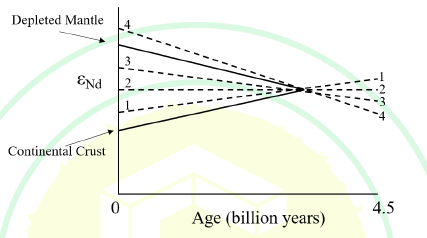
\includegraphics[width=0.6\columnwidth]{figs/fig6.png}
    \caption{}
    \label{fig:q30}
\end{figure}
\hfill{\brak{\text{GATE GG-1 2025}}}
\begin{enumerate}
\begin{multicols}{2}
    \item Line 1
    \item Line 2
    \item Line 3
    \item Line 4
\end{multicols}
\end{enumerate}

\item Which one of the following expressions represents porosity of a rock? \hfill{\brak{\text{GATE GG-1 2025}}}
\begin{enumerate}
    \item \brak{Solid volume - Pore volume} / Solid volume
    \item \brak{Bulk volume - Pore volume} / Bulk volume
    \item \brak{Bulk volume - Solid volume} / Solid volume
    \item \brak{Bulk volume - Solid volume} / Bulk volume
\end{enumerate}

\item Choose the correct option where both organisms do NOT secrete any $CaCO_3$ \brak{calcite or aragonite}. \hfill{\brak{\text{GATE GG-1 2025}}}
\begin{enumerate}
    \begin{multicols}{2}
    \item Foraminifera and Coccolithophore
    \item Diatom and Radiolaria
    \item Diatoms and Corals
    \item Foraminifera and Radiolaria
    \end{multicols}
\end{enumerate}

\item From the following optical properties of minerals, select an appropriate option to identify the direction of analyzer and polarizer if the available microscope is without a cross-hair. \hfill{\brak{\text{GATE GG-1 2025}}}
\begin{enumerate}
    \item Pleochroism of common hornblende
    \item Extinction of diopside
    \item Extinction of glaucophane
    \item Pleochroism of biotite
\end{enumerate}

\item Which one of the following minerals has crystallographic axes $a1=a2 \ne c$ and all interaxial angles equal to $90\degree$? \hfill{\brak{\text{GATE GG-1 2025}}}
\begin{enumerate}
    \begin{multicols}{4}
    \item Beryl
    \item Zircon
    \item Plagioclase
    \item Quartz
    \end{multicols}
\end{enumerate}

\item Which one of the following statements correctly describes the features in the geological map?
\begin{figure}[H]
    \centering
    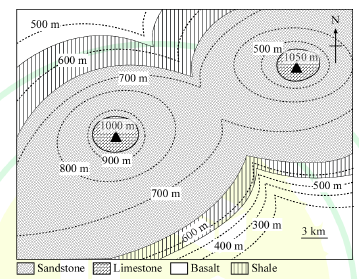
\includegraphics[width=0.8\columnwidth]{figs/fig7.png}
    \caption{}
    \label{fig:q35}
\end{figure}
\hfill{\brak{\text{GATE GG-1 2025}}}
\begin{enumerate}
    \item Horizontal sedimentary beds above a basalt basement
    \item Anticline consisting of sedimentary rocks and basalt
    \item Syncline consisting of sedimentary rocks and basalt
    \item Steep south-dipping sedimentary beds above a basalt basement
\end{enumerate}

\item In which one of the following rivers does helical flow play an important role in controlling river dynamics and channel morphology? \hfill{\brak{\text{GATE GG-1 2025}}}
\begin{enumerate}
    \begin{multicols}{2}
    \item Meandering rivers
    \item Straight rivers
    \item Braided rivers
    \item Bedrock rivers
    \end{multicols}
\end{enumerate}

\item Which of the following statements is/are NOT correct for stratigraphy of the Himalaya? \hfill{\brak{\text{GATE GG-1 2025}}}
\begin{enumerate}
    \item Tethyan Sedimentary Sequence rocks are of Precambrian age
    \item Lesser Himalayan Sequence rocks are younger than the Higher Himalayan Crystallines
    \item The Sub-Himalayan Sequence rocks are younger than the Lesser Himalayan rocks
    \item Collisional Himalayan orogeny occurred in the Cenozoic Era
\end{enumerate}

\item Which of the following factors will REDUCE the chances of landslide failure? \hfill{\brak{\text{GATE GG-1 2025}}}
\begin{enumerate}
    \item Increase in shear stress
    \item Increase in water content of pore spaces
    \item Increase in angle of internal friction
    \item Increase in cohesion of soil grains
\end{enumerate}

\item Which of the following rock and texture combinations is/are CORRECT? \hfill{\brak{\text{GATE GG-1 2025}}}
\begin{enumerate}
\begin{multicols}{2}
    \item Komatiite and Spinifex
    \item Gabbro and Ophitic
    \item Marble and Granoblastic
    \item Basalt and Porphyroblastic
\end{multicols}
\end{enumerate}

\item Which of the following statements regarding marine organisms is/are NOT true? \hfill{\brak{\text{GATE GG-1 2025}}}
\begin{enumerate}
    \item Foraminifera are multicellular marine organisms
    \item Sponges form their spicules with silica
    \item Coccolithophores are sea-surface dwelling organisms
    \item Species diversity of benthic foraminifera is less than that of planktonic foraminifera
\end{enumerate}

\item Which of the following rocks is/are characteristic of fossil subduction zones? \hfill{\brak{\text{GATE GG-1 2025}}}
\begin{enumerate}
    \item Wollastonite and scapolite bearing skarn
    \item Andalusite and staurolite bearing hornfels
    \item Garnet and glaucophane bearing blueschist
    \item Garnet and omphacite bearing eclogite
\end{enumerate}

\item Compared to $Fe$, $Mg$, and $Ca$, the content of $K$ is extremely low in igneous clinopyroxene. Which of the following CANNOT explain its low abundance? \hfill{\brak{\text{GATE GG-1 2025}}}
\begin{enumerate}
    \item $K^{+}$ has a larger ionic radius than $Fe^{2+}$, $Mg^{2+}$ and $Ca^{2+}$
    \item $K$ is incompatible and hence, enriched in the continental crust
    \item $K$ is fluid mobile and hence, easily leached out of clinopyroxene
    \item $K$ has multiple oxidation states
\end{enumerate}

\item The sediment yield at the outlet of a river having a catchment area of $8 \text{ km}^2$ is $6000 \text{ tons/year}$. If the sediment density is $1.5\, g/cm^3$, the average erosion rate of the river basin is \rule{3cm}{0.15mm} $mm/yr$. \brak{\text{Round off to two decimal places}} \hfill{\brak{\text{GATE GG-1 2025}}}

\item In a hypothetical rock, the $K_d$ values of element E in minerals M1, M2, and M3 are $1.5$, $1.0$, and $0.5$, respectively. The modal abundances of M1, M2, and M3 are $10\%$, $40\%$, and $50\%$, respectively. The bulk partition coefficient of element E in this rock is \rule{3cm}{0.15mm}. \brak{\text{Round off to two decimal places}} \hfill{\brak{\text{GATE GG-1 2025}}}

\item A particular Index of Alteration \brak{IA} is defined as the molar concentration ratio \brak{expressed as weight percentage} of fluid immobile element\brak{s} to fluid mobile element\brak{s} and is expressed by $100 \times \brak{[Al_2O_3] / \cbrak{[Al_2O_3] + [Na_2O] + [K_2O]}}$. For chemical weathering of silicate rocks, which one of the following statements is correct? \hfill{\brak{\text{GATE GG-1 2025}}}
\begin{enumerate}
    \item High IA values $\brak{> 85}$ indicate intense chemical weathering
    \item Low IA values $\brak{< 15}$ indicate intense chemical weathering
    \item The IA values do not vary for silicate rocks
    \item The minimum IA value for an unweathered granite is $0$
\end{enumerate}

\item What is the value of the maximum shear stress in a rock, for which the state of stress is given by the following Mohr circle?
\begin{figure}[H]
    \centering
    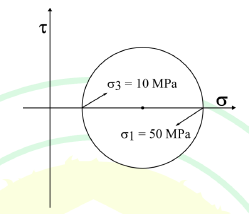
\includegraphics[width=0.5\columnwidth]{figs/fig8.png}
    \caption{}
    \label{fig:q46}
\end{figure}
\hfill{\brak{\text{GATE GG-1 2025}}}
\begin{enumerate}
\begin{multicols}{4}    
    \item $20\,MPa$
    \item $40\,MPa$
    \item $50\,MPa$
    \item $60\,MPa$
\end{multicols}
\end{enumerate}

\item In a hypothetical scenario, the element $Y$ has $4$ stable isotopes $^{197}Y$, $^{198}Y$, $^{199}Y$ and $^{200}Y$. The isotope $^{199}Y$ is radiogenic and is formed by $\beta^-$ decay of the isotope $^{199}X$ of the element $X$ with a half-life of $3.51$ billion years. An igneous rock, which has behaved as a closed system, has three different minerals P, Q, and R, which crystallized from the same magma $2$ billion years ago, with initial $X/Y$ ratios of $1.75$, $2.05$, and $0.75$, respectively. Which one of the following statements is true for the ratio $^{199}Y/^{200}Y$ in this igneous rock in the present day? \hfill{\brak{\text{GATE GG-1 2025}}}
\begin{enumerate}
\begin{multicols}{4} 
    \item $P > Q > R$
    \item $R > P > Q$
    \item $Q > P > R$
    \item $Q > R > P$
\end{multicols}
\end{enumerate}

\item Which one of the following factors governs the inclination of the slip face \brak{leeward side} of ripples? \hfill{\brak{\text{GATE GG-1 2025}}}
\begin{enumerate}
    \item Velocity of the transporting medium
    \item Internal friction angle
    \item Sediment supply
    \item Drag force
\end{enumerate}

\item High intensity rainfall in the Higher Himalayan region causes extensive damage, because of its large droplet size. Which one of the following relationships between the kinetic energy of raindrop \brak{E} and droplet diameter \brak{D} explains this process? \hfill{\brak{\text{GATE GG-1 2025}}}
\begin{enumerate}
\begin{multicols}{4} 
    \item $E \propto D^{1/2}$
    \item $E \propto D^2$
    \item $E \propto D^3$
    \item $E \propto D^4$
\end{multicols}
\end{enumerate}

\item The units A to H marked on the figure represent different rock formations. Select the option that describes the chronological sequence from old to young.
\begin{figure}[H]
    \centering
    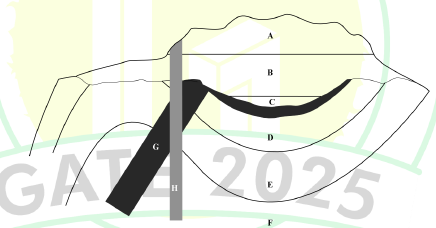
\includegraphics[width=0.7\columnwidth]{figs/fig9.png}
    \caption{}
    \label{fig:q50}
\end{figure}
\hfill{\brak{\text{GATE GG-1 2025}}}
\begin{enumerate}
\begin{multicols}{2} 
    \item F, E, D, G, C, B, A, H
    \item F, E, D, C, B, A, G, H
    \item F, E, D, G, C, H, B, A
    \item F, E, D, H, G, C, B, A
    \end{multicols}
\end{enumerate}

\item In the IUGS classification diagram for mafic and ultramafic rocks shown below, choose the correct option for the rocks labelled X and Y.
\begin{figure}[H]
    \centering
    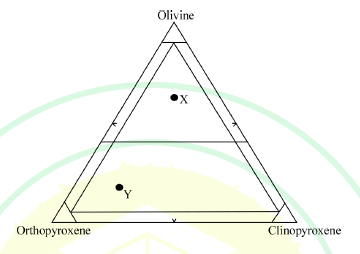
\includegraphics[width=0.6\columnwidth]{figs/fig10.png}
    \caption{}
    \label{fig:q51}
\end{figure}
\hfill{\brak{\text{GATE GG-1 2025}}}
\begin{enumerate}
    \item X: Harzburgite and Y: Olivine Websterite
    \item X: Lherzolite and Y: Olivine Websterite
    \item X: Dunite and Y: Clinopyroxenite
    \item X: Anorthosite and Y: Wehrlite
\end{enumerate}

\item Choose the correct combination of minerals \brak{listed in Group A} with the corresponding locations of their deposits \brak{listed in Group B}.
\begin{multicols}{2}
            \underline{\textbf{Group-A}}
            \begin{enumerate}[start =13]
                \item Magnesite
                \item Uraninite
                \item Clay minerals
                \item Platinum group elements
            \end{enumerate}

            \columnbreak

            \underline{\textbf{Group-B}}
            \begin{enumerate}
                \item Bikaner
                \item Nausahi
                \item Salem
                \item Jaduguda
            \end{enumerate}
        \end{multicols}
\hfill{\brak{\text{GATE GG-1 2025}}}
\begin{enumerate}
    \item M-$1$; N-$2$; O-$3$; P-$4$
    \item M-$4$; N-$3$; O-$2$; P-$1$
    \item M-$3$; N-$4$; O-$1$; P-$2$
    \item M-$2$; N-$4$; O-$1$; P-$3$
\end{enumerate}

\item Choose the explanation\brak{s} for negative $Eu$ anomalies in upper crustal rocks like granite and granodiorite. \hfill{\brak{\text{GATE GG-1 2025}}}
\begin{enumerate}
    \item These rocks are end-products of magmatic differentiation
    \item These rocks were formed by melting of the mantle, which was already depleted in $Eu$
    \item Most of the $Eu$ was incorporated in other minerals
    \item The melt residues contain plagioclase which are enriched in $Eu$
\end{enumerate}

\item Which characteristic feature\brak{s} best explain\brak{s} the HIMU mantle reservoir? \hfill{\brak{\text{GATE GG-1 2025}}}
\begin{enumerate}
    \item Magmas derived from this reservoir have high $^{208}Pb/^{204}Pb$ and $^{206}Pb/^{204}Pb$
    \item Magmas derived from this reservoir have high $^{207}Pb/^{204}Pb$ and $^{206}Pb/^{204}Pb$
    \item This reservoir has evolved with high $Th/U$
    \item This reservoir has evolved with high $U/Pb$
\end{enumerate}

\item Choose the correct option\brak{s} related to tectonic settings and associated rock types. \hfill{\brak{\text{GATE GG-1 2025}}}
\begin{enumerate}
    \item Tholeiitic basalts and alkali basalts are both associated with mid-oceanic ridges
    \item Andesites are commonly found in convergent plate boundaries
    \item Tholeiitic basalts and alkali basalts can both be associated with plume-related volcanism
    \item Volcanic rocks from subduction zones have high volatile content
\end{enumerate}

\item Which of the following options is/are correct for movement of warm-base glaciers? \hfill{\brak{\text{GATE GG-1 2025}}}
\begin{enumerate}
    \item Movement is dominated by basal sliding
    \item Internal deformation involving slippage within and between ice crystals leads to glacial movement
    \item Internal deformation is governed by shear stress following Power Law
    \item Vertical profile of glacier flow velocity is maximum at the base and decreases upwards
\end{enumerate}

\item Choose the correct option\brak{s} that describe\brak{s} the properties of clay minerals. \hfill{\brak{\text{GATE GG-1 2025}}}
\begin{enumerate}
    \item Kaolinite is two-layered
    \item Illite is two-layered
    \item Montmorillonite is two-layered
    \item Montmorillonite swells in contact with water
\end{enumerate}

\item Which of the following statements is/are correct for electromagnetic \brak{EM} radiation? \hfill{\brak{\text{GATE GG-1 2025}}}
\begin{enumerate}
    \item At room temperature, natural objects emit EM radiation
    \item Blackbody radiation is proportional to square of the absolute temperature of the body
    \item Wien's displacement law provides the dominant wavelength of EM emission
    \item EM energy decreases with increase in wavelength
\end{enumerate}

\item Which of the following options can be linked to rise in $CO_2$ concentration in the atmosphere? \hfill{\brak{\text{GATE GG-1 2025}}}
\begin{enumerate}
    \item Rise in seawater pH and sea surface temperature
    \item Decrease in seawater pH and and increase in bicarbonate ion concentration in seawater
    \item Warming of surface ocean water and decrease in carbonate ion concentration in seawater
    \item Decrease in seawater pH and decrease in bicarbonate ion concentration in seawater
\end{enumerate}

\item A sediment core of $4\,cm$ diameter and $35.81\,cm$ height was collected. This core had an initial weight of $1000.00\,g$ and upon drying the sediment, the weight decreased by $133.75\,g$. This core has a void ratio of $0.42857$, where void ratio is defined as the ratio of volume of void to the volume of solid $\brak{V_v/V_s}$. The average density of the sediment in the core is \rule{3cm}{0.15mm} $g/cm^3$. \brak{\text{Round off to two decimal places}} \hfill{\brak{\text{GATE GG-1 2025}}}

\item On a normal fault plane dipping $60\degree$ towards east, the measured heave and throw are $5\,m$ and $12\,m$, respectively. If the strike-slip component of the fault is $13\,m$, the magnitude of true displacement of the fault is \rule{3cm}{0.15mm} $m$. \brak{\text{Round off to one decimal place}} \hfill{\brak{\text{GATE GG-1 2025}}}

\item In the isochemical phase diagram shown below, the curved arrow represents the P-T path. The variance at peak metamorphism is \rule{3cm}{0.15mm}. \brak{\text{Answer in integer}}
\begin{figure}[H]
    \centering
    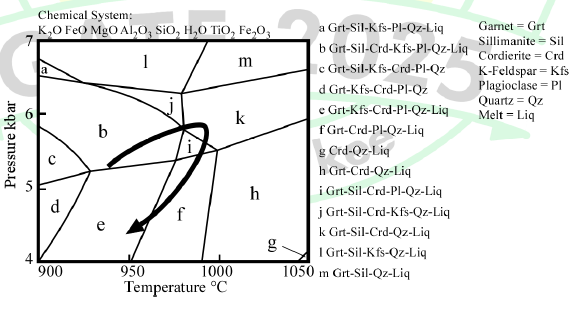
\includegraphics[width=0.8\columnwidth]{figs/fig11.png}
    \caption{}
    \label{fig:q62}
\end{figure}
\hfill{\brak{\text{GATE GG-1 2025}}}

\item A $3 \times 3$ image \brak{Image A} has been linearly stretched to get the maximum contrast in an $8$-bit display system. Digital Number \brak{DN} values of the pixels in Image A are shown. The value of the pixel marked as '?' in the output Image B after linear stretching is \rule{3cm}{0.15mm}. \brak{\text{Answer in integer}}
\begin{figure}[H]
    \centering
    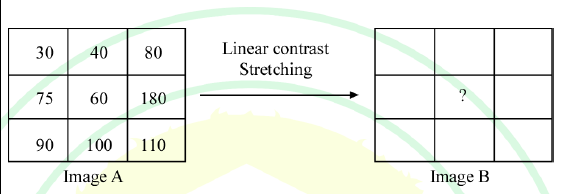
\includegraphics[width=0.7\columnwidth]{figs/fig12.png}
    \caption{}
    \label{fig:q63}
\end{figure}
\hfill{\brak{\text{GATE GG-1 2025}}}

\item $^{230}Th$ and $^{226}Ra$ are intermediate nuclides in the decay series of $^{238}U$ to $^{206}Pb$. The half-lives of $^{238}U$, $^{230}Th$ and $^{226}Ra$ are $4.47$ billion years, $75,000$ years, and $1600$ years, respectively. At secular equilibrium, when activities are equal, $10$ billion atoms of $^{238}U$ are present. The number of atoms of $^{226}Ra$ present at equilibrium is \rule{3cm}{0.15mm}. \brak{\text{Answer in integer}} \hfill{\brak{\text{GATE GG-1 2025}}}

\item The following table provides the mineral chemistry of a garnet. All oxides are in weight percentage and cations in atoms per formula unit. Total oxygen is taken as $12$ based on the ideal garnet formula. Consider $Fe$ as $Fe^{\text{total}}$ and $Fe^{3+}=0$. The $X_{pyrope}$ of this garnet is \rule{3cm}{0.15mm}. \brak{\text{Round off to three decimal places and do not multiply by hundred}}
\begin{table}[H]
    \centering
    \begin{center}
\begin{tabular}{ll}
    \textbf{Group I} & \textbf{Group II} \\
    P. Ferrite & 1. Hexagonal Close Packed (HCP) \\
    Q. Austenite & 2. Body Centered Cubic (BCC) \\
    R. Martensite & 3. Body Centered Tetragonal (BCT) \\
    & 4. Face Centered Cubic (FCC)
\end{tabular}
\end{center}
    \caption{Q.65}    
    \label{tab:placeholder}
\end{table}
\hfill{\brak{\text{GATE GG-1 2025}}}

\end{enumerate}
\end{document}
